\documentclass[11pt]{article}

% --- Mandatory Packages ---
\usepackage{amsmath}
\usepackage{amssymb}
\usepackage{amsthm}
\usepackage{geometry}
\usepackage{tikz}
\usetikzlibrary{arrows.meta, positioning, shapes}
\usepackage{mathrsfs}
\usepackage{mathtools}
\usepackage{hyperref}

% --- Page Geometry ---
\geometry{letterpaper, margin=1in}

% --- Theorem Environments ---
\newtheorem{theorem}{Theorem}[section]
\newtheorem{lemma}[theorem]{Lemma}
\newtheorem{proposition}[theorem]{Proposition}
\newtheorem{definition}[theorem]{Definition}
\newtheorem{corollary}[theorem]{Corollary}
\newtheorem{axiom}[theorem]{Axiom}

\title{\textbf{Homework 4: Proofs Involving Sets}}
\author{Tashfeen Omran}
\date{September 2026}

\begin{document}

\maketitle
\tableofcontents
\newpage

% ==============================================================================
% PART 1: Comprehensive Introduction, Context, and Prerequisites
% ==============================================================================
\section{Part 1: Comprehensive Introduction, Context, and Prerequisites}

\subsection{Conceptual Introduction: The Architecture of Sets}
In abstract mathematics, set theory serves as the foundational grammar through which all other mathematical structures (e.g., topological spaces, probability measures, algebraic rings) are articulated. This chapter, \textit{Proofs Involving Sets}, shifts the focus away from computational arithmetic toward formal logic and abstract containment. We define sets not merely as collections of objects, but as rigorously bounded mathematical entities governed by strict axioms. A fundamental principle explored here is how we formally prove that two sets are identical or how one set is nested within another.

\subsection{Core Concepts, Axioms, and Notation}
\begin{itemize}
    \item \textbf{Set Membership:} Denoted as $x \in A$, meaning element $x$ belongs to set $A$.
    \item \textbf{Subset ($\subseteq$):} $A \subseteq B$ if and only if $\forall x (x \in A \implies x \in B)$.
    \item \textbf{Set Equality ($=$):} By the Axiom of Extensionality, $A = B$ if and only if they contain the exact same elements. In practice, this is proven via \textit{mutual inclusion}: $A \subseteq B \land B \subseteq A$.
    \item \textbf{Union ($\cup$):} $A \cup B = \{x : x \in A \lor x \in B\}$.
    \item \textbf{Intersection ($\cap$):} $A \cap B = \{x : x \in A \land x \in B\}$.
    \item \textbf{Set Difference ($- \text{ or } \setminus$):} $A - B = \{x : x \in A \land x \notin B\}$.
    \item \textbf{Disjoint Sets:} $A$ and $B$ are disjoint if $A \cap B = \emptyset$.
\end{itemize}

\subsection{Intuition and Set-Theoretic / Logical Foundations}
To prove properties about abstract sets, mathematicians employ a technique colloquially known as \textbf{element-chasing}. Rather than looking at the set as a monolithic whole, we take an arbitrary, representative element (let's call it $x$) from the left-hand side of our proposition and use logical equivalences to ``chase'' it over to the right-hand side. We heavily rely on propositional logic—mapping unions to logical OR ($\lor$), intersections to logical AND ($\land$), and complements to logical NOT ($\neg$).

\subsection{Historical Context and Motivation}
In the late 19th century, Georg Cantor introduced ``naive set theory.'' However, this informal approach allowed for any conceivable property to define a set, which led to devastating paradoxes, most notably \textbf{Russell's Paradox} ($R = \{x : x \notin x\}$). If $R \in R$, then by definition $R \notin R$. If $R \notin R$, then by definition $R \in R$. This foundational crisis necessitated a rigorous axiomatic rebuild, culminating in the Zermelo-Fraenkel set theory with the Axiom of Choice (ZFC). Today, the proofs we conduct are descendants of this formalist rigor, ensuring no paradoxes can infiltrate our mathematical systems.

\subsection{Key Theorems, Lemmas, and Formulas}
\begin{theorem}[De Morgan's Laws for Sets]
For any sets $A$ and $B$ within a universal set $U$:
\[ (A \cup B)^c = A^c \cap B^c \quad \text{and} \quad (A \cap B)^c = A^c \cup B^c \]
\end{theorem}
\begin{theorem}[Distributive Laws]
For any sets $A, B,$ and $C$:
\[ A \cap (B \cup C) = (A \cap B) \cup (A \cap C) \quad \text{and} \quad A \cup (B \cap C) = (A \cup B) \cap (A \cup C) \]
\end{theorem}

\subsection{Prerequisites}
Mastery of this chapter requires a strong command of:
\begin{enumerate}
    \item \textbf{Propositional Logic:} Truth tables, implication ($P \implies Q$), and logical equivalences.
    \item \textbf{Proof Techniques:} Direct proof, proof by contradiction, and proof by contrapositive.
    \item \textbf{Modular Arithmetic:} Understanding equivalence classes, e.g., $a \equiv b \pmod n \iff n \mid (a - b)$.
\end{enumerate}

% ==============================================================================
% PART 2: Detailed Homework Solutions
% ==============================================================================
\section{Part 2: Detailed Homework Solutions (Rigorous Proofs)}

To ensure comprehensive mastery, the following problems have been strategically selected from Section 4.4 to cover all distinct archetypes of set-theoretic proofs.

\subsection{Problem 4.40 (Archetype: Mutual Inclusion and Set Partitions)}
\textbf{Statement:} Let $A$ and $B$ be sets. Prove that $A \cup B = (A - B) \cup (B - A) \cup (A \cap B)$.

\begin{proof}[\textbf{Proof Technique: Direct Proof via Mutual Inclusion}]
We must demonstrate two subset inclusions: $A \cup B \subseteq (A - B) \cup (B - A) \cup (A \cap B)$ and $(A - B) \cup (B - A) \cup (A \cap B) \subseteq A \cup B$.

\textbf{Part 1: Forward Inclusion} ($\subseteq$) \\
Let $x$ be an arbitrary element such that $x \in A \cup B$. 
By definition of set union, this implies $x \in A$ or $x \in B$. 
By the logical Law of the Excluded Middle, we know that either $x \in A$ or $x \notin A$, and independently, either $x \in B$ or $x \notin B$. Thus, we can evaluate the exhaustive scenarios for $x$:
\begin{itemize}
    \item \textit{Case 1:} Assume $x \in A$ and $x \notin B$. By definition of set difference, $x \in A - B$.
    \item \textit{Case 2:} Assume $x \notin A$ and $x \in B$. By definition of set difference, $x \in B - A$.
    \item \textit{Case 3:} Assume $x \in A$ and $x \in B$. By definition of set intersection, $x \in A \cap B$.
\end{itemize}
Note that the case $(x \notin A \text{ and } x \notin B)$ is impossible because it contradicts our starting premise $x \in A \cup B$. In all valid cases, $x$ belongs to at least one of the sets $(A - B)$, $(B - A)$, or $(A \cap B)$. 
Therefore, $x \in (A - B) \cup (B - A) \cup (A \cap B)$, which establishes $A \cup B \subseteq (A - B) \cup (B - A) \cup (A \cap B)$.

\textbf{Part 2: Reverse Inclusion} ($\supseteq$) \\
Conversely, let $y \in (A - B) \cup (B - A) \cup (A \cap B)$. 
By the definition of union, $y$ belongs to at least one of these three sets.
\begin{itemize}
    \item \textit{Case 1:} $y \in A - B \implies y \in A$ and $y \notin B \implies y \in A \implies y \in A \cup B$.
    \item \textit{Case 2:} $y \in B - A \implies y \in B$ and $y \notin A \implies y \in B \implies y \in A \cup B$.
    \item \textit{Case 3:} $y \in A \cap B \implies y \in A$ and $y \in B \implies y \in A \implies y \in A \cup B$.
\end{itemize}
Since $y \in A \cup B$ in every exhaustive case, $(A - B) \cup (B - A) \cup (A \cap B) \subseteq A \cup B$.
Having proven inclusion in both directions, we conclude $A \cup B = (A - B) \cup (B - A) \cup (A \cap B)$.
\end{proof}

\subsection{Problem 4.42 (Archetype: Biconditional Set Inclusion)}
\textbf{Statement:} Let $A$ and $B$ be sets. Prove that $A \cap B = A$ if and only if $A \subseteq B$.

\begin{proof}[\textbf{Proof Technique: Direct Proof of a Biconditional}]
We must prove both directions of the ``if and only if'' ($\iff$) statement.

\textbf{Direction 1: ($A \cap B = A \implies A \subseteq B$)} \\
Assume $A \cap B = A$. We aim to show $A \subseteq B$.
Let $x \in A$. Since we assumed $A = A \cap B$, substituting $A$ yields $x \in A \cap B$.
By the definition of set intersection, $x \in A \cap B$ means $x \in A$ and $x \in B$.
In particular, this entails that $x \in B$.
Since every arbitrary $x \in A$ is also an element of $B$, we conclude by definition that $A \subseteq B$.

\textbf{Direction 2: ($A \subseteq B \implies A \cap B = A$)} \\
Assume $A \subseteq B$. We aim to show $A \cap B = A$. We do this via mutual inclusion.
\textit{Sub-part a:} It is trivially true by the definition of intersection that for any sets, $A \cap B \subseteq A$. 
\textit{Sub-part b:} Now we show $A \subseteq A \cap B$. Let $y \in A$. Since we assumed $A \subseteq B$, it must follow that $y \in B$. Because $y \in A$ and $y \in B$, by definition $y \in A \cap B$. Therefore, $A \subseteq A \cap B$.
Since $A \cap B \subseteq A$ and $A \subseteq A \cap B$, we have proven $A \cap B = A$.
\end{proof}

\subsection{Problem 4.43 (Archetype: Counterexamples and Logical Elimination)}
\textbf{Statement:} 
(a) Give an example of three sets $A, B, C$ such that $A \cap B = A \cap C$ but $B \neq C$. \\
(b) Give an example of three sets $A, B, C$ such that $A \cup B = A \cup C$ but $B \neq C$. \\
(c) Prove that if $A \cap B = A \cap C$ and $A \cup B = A \cup C$, then $B = C$.

\begin{proof}[\textbf{Solutions and Proof}]
\textbf{Part (a):} Let $A = \emptyset$, $B = \{1\}$, and $C = \{2\}$. \\
Calculations: $A \cap B = \emptyset \cap \{1\} = \emptyset$. $A \cap C = \emptyset \cap \{2\} = \emptyset$. \\
Thus, $A \cap B = A \cap C$, but clearly $B \neq C$.

\textbf{Part (b):} Let $A = \{1, 2\}$, $B = \{1\}$, and $C = \{2\}$. \\
Calculations: $A \cup B = \{1, 2\} \cup \{1\} = \{1, 2\}$. $A \cup C = \{1, 2\} \cup \{2\} = \{1, 2\}$. \\
Thus, $A \cup B = A \cup C$, but clearly $B \neq C$.

\textbf{Part (c):} \textit{(Proof Technique: Direct Proof via Cases and Element-Chasing)} \\
Assume $A \cap B = A \cap C$ and $A \cup B = A \cup C$. We must show $B = C$ by mutual inclusion.
First, we show $B \subseteq C$. Let $x \in B$. 
Because $x \in B$, it immediately follows that $x \in A \cup B$. 
By our second assumption ($A \cup B = A \cup C$), we substitute to find $x \in A \cup C$. 
This means $x \in A$ or $x \in C$. We analyze both possibilities:
\begin{itemize}
    \item \textit{Case 1:} $x \in C$. Here, the desired result is immediately achieved.
    \item \textit{Case 2:} $x \in A$. Since we initially established $x \in B$, we now have $x \in A$ and $x \in B$, meaning $x \in A \cap B$. 
    By our first assumption ($A \cap B = A \cap C$), we substitute to find $x \in A \cap C$.
    By definition of intersection, this implies $x \in A$ and $x \in C$. Hence, $x \in C$.
\end{itemize}
In all possible cases, $x \in C$. Therefore, $B \subseteq C$.
By symmetry, if we start with $y \in C$, identical logic proves $y \in B$, yielding $C \subseteq B$.
Thus, $B = C$.
\end{proof}

\subsection{Problem 4.45 (Archetype: Number-Theoretic Sets)}
\textbf{Statement:} Let $A = \{n \in \mathbb{Z} : n \equiv 1 \pmod 2\}$ and $B = \{n \in \mathbb{Z} : n \equiv 3 \pmod 4\}$. Prove that $B \subseteq A$.

\begin{proof}[\textbf{Proof Technique: Direct Proof with Modular Algebra}]
Let $x \in B$. By the definition of set $B$, $x$ is an integer such that $x \equiv 3 \pmod 4$.
By the definition of modular congruence, this means $4 \mid (x - 3)$.
By the definition of divisibility, there exists some integer $k$ such that $x - 3 = 4k$.
We can isolate $x$ algebraically:
\[ x = 4k + 3 \]
We aim to show $x \in A$, which requires demonstrating $x \equiv 1 \pmod 2$. Let us manipulate the expression for $x$:
\[ x = 4k + 2 + 1 \]
\[ x - 1 = 4k + 2 \]
\[ x - 1 = 2(2k + 1) \]
Since integers are closed under multiplication and addition, $(2k + 1)$ is an integer. Let us define a new integer $m = 2k + 1$. We then have:
\[ x - 1 = 2m \]
This equation signifies that $2 \mid (x - 1)$, which by definition is mathematically identical to $x \equiv 1 \pmod 2$.
Therefore, $x$ satisfies the entry requirements for set $A$, meaning $x \in A$.
Since an arbitrary element $x \in B$ implies $x \in A$, we conclude $B \subseteq A$.
\end{proof}

\subsection{Problem 4.48 (Archetype: Combining Logic and Number Theory)}
\textbf{Statement:} Let $A = \{n \in \mathbb{Z} : 2 \mid n\}$ and $B = \{n \in \mathbb{Z} : 4 \mid n\}$. Let $n \in \mathbb{Z}$. Prove that $n \in A - B$ if and only if $n = 2k$ for some odd integer $k$.

\begin{proof}[\textbf{Proof Technique: Biconditional Proof (Direct and Contradiction)}]
\textbf{Direction 1 ($\implies$):} Assume $n \in A - B$. 
By definition, $n \in A$ and $n \notin B$. 
Because $n \in A$, $2 \mid n$, meaning there exists an integer $k$ such that $n = 2k$.
Because $n \notin B$, $4 \nmid n$. 
We must show that $k$ is an odd integer. We proceed by contradiction. 
Assume $k$ is an even integer. Then $k = 2m$ for some integer $m$. 
Substitute this into our formula for $n$:
\[ n = 2(2m) = 4m \]
This implies $4 \mid n$, forcing $n \in B$. This directly contradicts our premise that $n \notin B$. Thus, our assumption was false; $k$ must be an odd integer.

\textbf{Direction 2 ($\impliedby$):} Assume $n = 2k$ for some odd integer $k$.
Since $n = 2k$ and $k \in \mathbb{Z}$, $2 \mid n$, so $n \in A$.
Since $k$ is odd, $k = 2m + 1$ for some integer $m$. Substituting this gives:
\[ n = 2(2m + 1) = 4m + 2 \]
We must prove $n \notin B$ (i.e., $4 \nmid n$). Assume for contradiction that $4 \mid n$. Then $n = 4j$ for some integer $j$. We equate the two expressions for $n$:
\[ 4m + 2 = 4j \]
\[ 2 = 4j - 4m = 4(j - m) \]
Dividing by 2 yields:
\[ 1 = 2(j - m) \]
Since $j, m \in \mathbb{Z}$, $(j - m)$ is an integer. This equation implies that $1$ is an even integer, which is a mathematical absurdity. The contradiction implies $4 \nmid n$. 
Hence, $n \in A$ and $n \notin B$, which means $n \in A - B$.
\end{proof}

\subsection{Problem 4.51 (Archetype: Evaluating Logical Necessity)}
\textbf{Statement:} Let $A$ and $B$ be subsets of a universal set. Which of the following is a necessary condition for $A$ and $B$ to be disjoint? \\
(a) Either $A = \emptyset$ or $B = \emptyset$. \\
(b) Whenever $x \notin A$, it must occur that $x \in B$. \\
(c) Whenever $x \notin A$, it must occur that $x \notin B$. \\
(d) Whenever $x \in A$, it must occur that $x \in B$. \\
(e) Whenever $x \in A$, it must occur that $x \notin B$.

\begin{proof}[\textbf{Solution and Justification}]
By definition, $A$ and $B$ are disjoint if and only if their intersection is empty, $A \cap B = \emptyset$. This means there exists no element $x$ in the universal set $U$ that belongs to both $A$ and $B$ simultaneously. Formally:
\[ \neg \exists x \in U : (x \in A \land x \in B) \]
Equivalently, using the universal quantifier:
\[ \forall x \in U, \neg(x \in A \land x \in B) \]
By De Morgan's Law for logic, $\neg(P \land Q) \equiv \neg P \lor \neg Q$. Furthermore, the logical definition of implication states $P \implies Q \equiv \neg P \lor Q$. Setting $P$ as ``$x \in A$'' and $Q$ as ``$x \notin B$'', we can rewrite the disjointedness condition as:
\[ \forall x \in U, (x \in A \implies x \notin B) \]
Translating this mathematical logic into English yields: ``Whenever $x \in A$, it must occur that $x \notin B$.''
This matches option \textbf{(e)} perfectly. It is not just a necessary condition, but a necessary and sufficient condition.
\end{proof}

% ==============================================================================
% PART 3: In-Depth Analysis of Problems and Techniques
% ==============================================================================
\section{Part 3: In-Depth Analysis of Problems and Techniques}

\subsection{A) Problem Types and Logical Strategies}
The homework problems distill into three distinct archetypes:
\begin{enumerate}
    \item \textbf{Element-Chasing / Set Identity (e.g., 4.40, 4.42, 4.43c):} The strategy is universally to grab an arbitrary element $x$ from one side and deduce its presence in the other side via logical implications. If the claim is an equality ($A = B$), one must independently prove $A \subseteq B$ and $B \subseteq A$. 
    \item \textbf{Number-Theoretic Sets (e.g., 4.45, 4.48):} The focus shifts from pure logic to algebraic manipulation. The strategy requires instantly converting set notation into algebraic equations (e.g., $x \equiv a \pmod n \to x = nk + a$). Proving a negative condition ($4 \nmid n$) is usually best handled by \textit{Proof by Contradiction}.
    \item \textbf{Counterexamples (e.g., 4.43a, 4.43b):} Proving a universal claim false only requires one specific instance. The strategy is to choose the smallest, simplest sets possible (often $\emptyset, \{1\}, \{2\}$) to limit moving variables.
\end{enumerate}

\subsection{B) Key Analytical and Logical Manipulations}
\begin{itemize}
    \item \textbf{The Law of Excluded Middle ($P \lor \neg P$):} Utilized heavily in 4.40 to split the universe into cases (e.g., $x \in B$ or $x \notin B$). Without this, we cannot form exhaustive branches to evaluate unions and differences.
    \item \textbf{Implication Translation via De Morgan's:} Used in 4.51. Translating $\neg(x \in A \land x \in B)$ to $x \in A \implies x \notin B$ is a powerful tool to convert static set relationships into functional logical tests.
    \item \textbf{Odd/Even Parameterization Parity:} Used in 4.45 and 4.48. Factoring a $2$ out of an expression (e.g., $4m + 2 = 2(2m + 1)$) to isolate an algebraic definition is the primary bridge between modular sets.
\end{itemize}

% ==============================================================================
% PART 4: "Cheatsheet", Visuals, and Tips for Success
% ==============================================================================
\section{Part 4: ``Cheatsheet'', Visuals, and Tips for Success}

\subsection{Essential Logic-to-Set Dictionary}
\begin{center}
\begin{tabular}{|l|l|l|}
\hline
\textbf{Logic Symbol} & \textbf{Set Operation} & \textbf{Meaning in Element-Chasing} \\ \hline
$\land$ (AND) & $\cap$ (Intersection) & $x \in A \cap B \iff (x \in A) \land (x \in B)$ \\ \hline
$\lor$ (OR) & $\cup$ (Union) & $x \in A \cup B \iff (x \in A) \lor (x \in B)$ \\ \hline
$\neg$ (NOT) & $A^c$ or $U \setminus A$ & $x \in A^c \iff \neg(x \in A) \iff x \notin A$ \\ \hline
$\implies$ (Implies) & $\subseteq$ (Subset) & $A \subseteq B \iff (x \in A \implies x \in B)$ \\ \hline
$\iff$ (Biconditional) & $=$ (Equality) & $A = B \iff (x \in A \iff x \in B)$ \\ \hline
\end{tabular}
\end{center}

\subsection{Set Visualization: Disjoint Partitioning of Unions}
The visual below strictly corresponds to the result proven in \textbf{Problem 4.40}: $A \cup B$ can be uniquely partitioned into three mutually exclusive subsets: $A - B$, $A \cap B$, and $B - A$.

\begin{center}
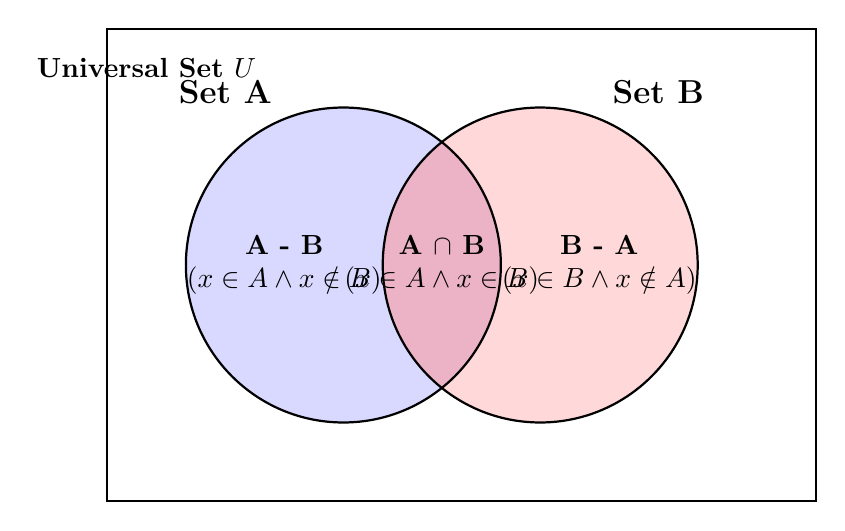
\begin{tikzpicture}
    % Draw universal set
    \draw[thick] (-3,-3) rectangle (6,3);
    \node at (-2.5, 2.5) {\textbf{Universal Set $U$}};

    % Draw A - B
    \begin{scope}
        \clip (0,0) circle (2);
        \fill[blue!15] (-3,-3) rectangle (3,3); 
        \fill[white] (2.5,0) circle (2); 
    \end{scope}

    % Draw B - A
    \begin{scope}
        \clip (2.5,0) circle (2);
        \fill[red!15] (-1,-3) rectangle (6,3); 
        \fill[white] (0,0) circle (2); 
    \end{scope}

    % Draw A \cap B
    \begin{scope}
        \clip (0,0) circle (2);
        \fill[purple!30] (2.5,0) circle (2); 
    \end{scope}

    % Outlines
    \draw[thick] (0,0) circle (2);
    \draw[thick] (2.5,0) circle (2);
    
    % Labels
    \node[align=center] at (-0.75, 0) {\textbf{A - B}\\$(x \in A \land x \notin B)$};
    \node[align=center] at (3.25, 0) {\textbf{B - A}\\$(x \in B \land x \notin A)$};
    \node[align=center] at (1.25, 0) {\textbf{A $\cap$ B}\\$(x \in A \land x \in B)$};
    
    \node at (-1.5, 2.2) {\large \textbf{Set A}};
    \node at (4, 2.2) {\large \textbf{Set B}};
\end{tikzpicture}
\end{center}

\subsection{Heuristics and Pitfalls}
\begin{itemize}
    \item \textbf{Heuristic ("The Unpacking Rule"):} Whenever you get stuck, unpack definitions. Do not stare at $x \in (A \setminus B)^c$. Immediately unpack it to $\neg(x \in A \land x \notin B) \implies x \notin A \lor x \in B$.
    \item \textbf{Pitfall (Assuming Non-Empty Sets):} When proving $A \subseteq B$, starting a proof with ``Let $x \in A$...'' inherently assumes $A$ is not empty. Technically, one must state ``If $A = \emptyset$, it is trivially a subset of $B$. Otherwise, let $x \in A\dots$''
    \item \textbf{Pitfall (Symmetric Errors):} Do not confuse ``$x \in A \implies x \in B$'' with ``$x \in B \implies x \in A$.'' This is the logical fallacy of Affirming the Consequent, which in set theory incorrectly assumes $A \subseteq B \implies B \subseteq A$.
\end{itemize}

% ==============================================================================
% PART 5: Conceptual Synthesis and The "Big Picture"
% ==============================================================================
\section{Part 5: Conceptual Synthesis and The ``Big Picture''}

\subsection{A) Thematic Connections: The Logic-Set Bridge}
The core theme of this topic is establishing an \textbf{isomorphism between propositional logic and set theory}. Every manipulation we perform on equations involving operators like $\cup, \cap,$ and $^c$ is a direct mirror of logical deductions using $\lor, \land,$ and $\neg$. This guarantees that set theory inherits the absolute rigor of formal logic, which is crucial because collections of objects are mathematically meaningless unless their bounds are perfectly logically defined.

\subsection{B) Forward Links: The Bedrock of Advanced Mathematics}
Understanding unions, intersections, and set inclusion is not the endgame; it is the starting line. 
\begin{itemize}
    \item \textbf{Topology:} Open and closed sets are defined entirely through infinite unions and finite intersections.
    \item \textbf{Measure Theory:} A $\sigma$-algebra (the collection of all events we can assign a probability to) is defined explicitly as a set closed under complementation and countable unions. 
    \item \textbf{Probability Theory:} Kolmogorov’s Axioms of Probability map directly to set operations. For mutually exclusive (disjoint) sets, $P(A \cup B) = P(A) + P(B)$. Without a mastery of set disjointness (as seen in Problem 4.51), advanced probability is impenetrable.
\end{itemize}

% ==============================================================================
% PART 6: Abstract Real-World Modeling
% ==============================================================================
\section{Part 6: Abstract Real-World Modeling (AI, ML, \& Quant Finance)}

\subsection{Concrete Scenarios}
\begin{enumerate}
    \item \textbf{Statistical Machine Learning (Evaluation Metrics):} In binary classification models, the Universe $U$ is the test dataset. Set $A$ is the ground truth (Actual Positives) and Set $B$ is the model output (Predicted Positives). Precision, Recall, and F1-Scores are entirely functions of the cardinalities of intersections ($A \cap B$) and differences ($B - A$).
    \item \textbf{Quantitative Finance (Stochastic Filtrations):} In Black-Scholes derivative pricing, information revealing over time is modeled via a ``filtration'' $\mathcal{F}_t$, which is an ascending sequence of $\sigma$-algebras ($\mathcal{F}_0 \subseteq \mathcal{F}_1 \dots \subseteq \mathcal{F}_T$). Knowing how to prove subset inclusions formally proves that information strictly grows over time.
\end{enumerate}

\subsection{Mathematical Model: The Binary Classifier Evaluation Space}
Let us formalize the evaluation of a Generative AI text-classifier designed to detect fraudulent financial documents. 

\textbf{Definition of the Space:} 
Let $U = \{d_1, d_2, \dots, d_N\}$ be our discrete finite state space (dataset) of documents. 
Let $T \subseteq U$ be the theoretical ``True Fraud'' set. 
Let $P \subseteq U$ be the ``Predicted Fraud'' set generated by our AI model parameterized by weights $\theta$.

\textbf{Modeling Set Theoretic Loss/Optimization:}
To optimize the AI, we need a mathematical function evaluating its accuracy. In ML, False Positives ($FP$) and False Negatives ($FN$) often carry different financial penalties ($\alpha$ and $\beta$). 
Using strict set definitions:
\[ FP = P - T = \{d \in U : d \in P \land d \notin T\} \]
\[ FN = T - P = \{d \in U : d \in T \land d \notin P\} \]

We can define a Loss Function $\mathcal{L}(\theta)$ based on the cardinality (size) of these set operations:
\[ \mathcal{L}(\theta) = \alpha |P - T| + \beta |T - P| \]
Notice that the total errors made by the model is the union of these two disjoint sets, which mathematically forms the \textit{Symmetric Difference} ($P \Delta T$). Minimizing this Set Difference is the literal mathematical equivalent of maximizing a model's predictive capability.

% ==============================================================================
% PART 7: Common Variations and Untested Concepts
% ==============================================================================
\section{Part 7: Common Variations and Untested Concepts}

The standard university curriculum on set theory rigorously tests the \textbf{Symmetric Difference}, an operation critically missing from the provided Section 4.4 homework list. 

\begin{definition}[Symmetric Difference]
The symmetric difference of sets $A$ and $B$, denoted $A \Delta B$, is the set of elements belonging to exactly one of the two sets: 
\[ A \Delta B = (A - B) \cup (B - A) \]
\end{definition}

\textbf{Untested Theorem Variation:} Prove that $A \Delta B = (A \cup B) - (A \cap B)$. 

\begin{proof}
Let $x \in A \Delta B$. By definition, $x \in (A - B) \cup (B - A)$.
This implies $(x \in A \land x \notin B)$ or $(x \in B \land x \notin A)$.
In both sub-cases, $x$ belongs to at least one set, meaning $x \in A \cup B$. 
Furthermore, in both sub-cases, it is impossible for $x$ to belong to \textit{both} sets simultaneously. Thus, $x \notin (A \cap B)$.
Since $x \in A \cup B$ and $x \notin A \cap B$, by definition of set difference, $x \in (A \cup B) - (A \cap B)$.

Conversely, let $y \in (A \cup B) - (A \cap B)$. 
This means $y \in A \cup B$ AND $y \notin A \cap B$. 
Because $y \in A \cup B$, we know $y \in A$ or $y \in B$. 
Because $y \notin A \cap B$, by De Morgan's Law, $y \notin A$ or $y \notin B$. 
Therefore, if $y \in A$, then it must be that $y \notin B$ (yielding $y \in A - B$). If $y \in B$, then it must be that $y \notin A$ (yielding $y \in B - A$).
In either valid scenario, $y \in (A - B) \cup (B - A)$, which is $A \Delta B$. 
Thus, the equality holds.
\end{proof}

% ==============================================================================
% PART 8: Advanced Diagnostic Testing: "Find the Flaw"
% ==============================================================================
\section{Part 8: Advanced Diagnostic Testing: ``Find the Flaw''}
\textit{Instructions: Each problem below contains a subtle logical fallacy or mathematical trap. Your task is to act as the grader: identify the flaw, explain the violation, and reference the Solution Key at the bottom for verification.}

\subsection{Flawed Problem 1: Subset Distributions}
\textbf{Claim:} For any sets $A, B$, and $C$, if $A \subseteq (B \cup C)$, then $A \subseteq B$ or $A \subseteq C$. \\
\textbf{Proof:} Let $x \in A$. Because $A \subseteq (B \cup C)$, it follows that $x \in B \cup C$. By definition of union, $x \in B$ or $x \in C$. 
If $x \in B$, then $A \subseteq B$. If $x \in C$, then $A \subseteq C$. Therefore, $A \subseteq B$ or $A \subseteq C$. $\blacksquare$

\subsection{Flawed Problem 2: Set Equality via Circular Logic}
\textbf{Claim:} For sets $A$ and $B$, if $A \cup B = A$, then $B \subseteq A$. \\
\textbf{Proof:} Assume $A \cup B = A$. We must prove $B \subseteq A$. Let $x \in B$. Since a set is always a subset of its union with another set, $B \subseteq A \cup B$. Thus, $x \in A \cup B$. Since we assumed $B \subseteq A$ for our proof, it follows that $x \in A$. Therefore, $B \subseteq A$. $\blacksquare$

\subsection{Flawed Problem 3: Modulo Disjunction Trap}
\textbf{Claim:} Let $S = \{x \in \mathbb{Z} : x^2 \equiv 1 \pmod 4\}$. If $a \in S$, then $a \equiv 1 \pmod 4$. \\
\textbf{Proof:} Let $a \in S$. By definition, $a^2 \equiv 1 \pmod 4$, meaning $4 \mid (a^2 - 1)$. Factoring the expression yields $4 \mid (a - 1)(a + 1)$. Since $4$ divides the product, it must divide one of the factors. Therefore, either $4 \mid (a - 1)$ or $4 \mid (a + 1)$. If $4 \mid (a - 1)$, then $a \equiv 1 \pmod 4$, completing the proof. $\blacksquare$

\subsection{Flawed Problem 4: Visual Proof Legitimacy}
\textbf{Claim:} $A - (B \cup C) = (A - B) \cap (A - C)$. \\
\textbf{Proof:} Draw three intersecting circles representing sets A, B, and C in a Venn diagram. Shade the region for $A$. Erase the circles for $B$ and $C$. The remaining shaded portion is only the part of $A$ entirely outside both $B$ and $C$. If we shade $A-B$ and intersect it with the shading for $A-C$, we get the same image. Because the drawings match perfectly, the sets are equal. $\blacksquare$

\subsection{Flawed Problem 5: Intersection De Morgan Error}
\textbf{Claim:} $(A - B)^c = A^c \cap B$. \\
\textbf{Proof:} The set $A - B$ is defined logically as $\{x : x \in A \land x \notin B\}$. We take the complement of the entire set, which means applying a logical negation. $\neg(x \in A \land x \notin B)$. By De Morgan's Law, we distribute the negation and flip the sign: $\neg(x \in A) \land \neg(x \notin B)$. This evaluates to $x \notin A \land x \in B$. This means $x \in A^c \cap B$. $\blacksquare$

% --- Solution Key ---
\vspace{1cm}
\hrule
\vspace{0.5cm}
\subsection*{Solution Key: Resolutions to Flawed Proofs}
\begin{itemize}
    \item \textbf{Resolution 1:} The flaw occurs when leaping from ``a specific $x \in B$ or $C$'' to ``the entirety of $A \subseteq B$ or $C$''. Set $A$ might have half its elements in $B$ and half in $C$. Counterexample: $A = \{1, 2\}, B = \{1\}, C = \{2\}$. $A \subseteq B \cup C$ holds, but neither $A \subseteq B$ nor $A \subseteq C$ is true.
    \item \textbf{Resolution 2:} Circular reasoning (Begging the Question). In the middle of the proof, the author writes ``Since we assumed $B \subseteq A$ for our proof...'' This is what they were tasked with proving! The correct deduction from $x \in A \cup B$ is to substitute the given premise $A \cup B = A$, which directly yields $x \in A$.
    \item \textbf{Resolution 3:} The flaw is assuming $4$ is prime. The rule ``if $p \mid xy$, then $p \mid x$ or $p \mid y$'' \textit{only} holds when $p$ is a prime number. Since $4 = 2 \times 2$, it is possible that $2 \mid (a-1)$ and $2 \mid (a+1)$ without $4$ dividing either independently. Counterexample: let $a = 3$. $3^2 = 9 \equiv 1 \pmod 4$, but $3 \not\equiv 1 \pmod 4$.
    \item \textbf{Resolution 4:} A Venn Diagram is an illustration, not a rigorous mathematical proof. It inherently assumes general position (that all intersections exist and sets are non-empty), which fails to cover boundary cases like empty sets or sets containing sets. It does not replace the requirement for formal element-chasing. 
    \item \textbf{Resolution 5:} Improper application of De Morgan's Law. $\neg(P \land Q) \equiv \neg P \lor \neg Q$. The author incorrectly kept the AND ($\land$) symbol. The correct negation of $(x \in A \land x \notin B)$ is $(x \notin A) \lor (x \in B)$, meaning $(A - B)^c = A^c \cup B$. 
\end{itemize}

\end{document}